%\subsection{Development}
%
%The contract was developed using Ethereum's Remix client \cite{remix}. This allowed me to quickly debug compile and runtime errors, as well as calling functions with ease. I ran the Ganache \cite{ganache} desktop application to provide Remix with a test blockchain, and accessed accounts and made payments through MetaMask \cite{metamask}.
%
%To test the game with multiple players, I ran both Firefox and Chrome web browsers (each with separate MetaMask instances), and shared the contract address between them. Each MetaMask instance was utilising a different Ethereum account.
%
%I maintained a git repository containing the contract to help with version control, stored at https://github.com/louisdeb/dapp-poker.

\subsection{Game Logic}

\subsubsection{Joining and Starting the Game}

One player creates the contract. Then he, and any other players with the address of the contract, may call \texttt{joinGame}. Between 2 and 7 players are allowed to partake in a single game.

Once there are sufficient players in the game, the owner can call \texttt{startGame} which shuffles the deck, and assigns the current player to the one paying the small blind.

\subsubsection{Making Bets}

The small blind, and the player to his right, the big blind, must call \texttt{paySmallBlind} and \texttt{payBigBlind} respectively, in order. Once the blinds have been paid, the cards are dealt. The blinds are predetermined in the contract as:

\begin{enumerate}[$\bullet$]
\item Small Blind: 1 finney
\item Big Blind: 2 finney \footnote{A possible extension of this project would be to allow the owner to set these values on creating the contract (though the big blind is always twice the small blind). Then players could check the blind values before joining a game and see if the stakes suit what they want to bet.}
\end{enumerate}

At every round of betting, we allow each player the chance to raise, call or fold. Raising and calling are done through the public, payable function \texttt{makeBet}. If the bet is not sufficient to call the current bet, the transaction is reverted. The \texttt{makeBet} function is implemented as follows:

\begin{lstlisting}
function makeBet() public payable onlyCurrentPlayer whenPlaying whenDealt {
  uint newBet = bets[msg.sender] + msg.value;
  if(newBet < maxBet)
   revert();

  bets[msg.sender] = newBet;
  setMaxBet(bets[msg.sender], msg.sender);
  incrementCurrentPlayer();
  tryIncrementRound();
}
\end{lstlisting}

The implementation is simple and easy to follow. Function call \texttt{incrementCurrentPlayer()} moves the play to the next player round the table. \texttt{tryIncrementRound()} will check whether all players, who have not folded, have matched the maximum bet, and that all players have had the chance to raise (tracked through the variable \texttt{lastPlayerToRaise}).

We can see the logic of setting a maximum bet and setting the last player to raise in the function, \texttt{setMaxBet}:

\begin{lstlisting}
function setMaxBet(uint bet, address sender) private {
  if (bet > maxBet) {
      maxBet = bet;
      lastPlayerToRaise = sender;
  }
}
\end{lstlisting}

Then, we only try to increment the round (in \texttt{tryIncrementRound}) if the following condition is met:

\begin{lstlisting}
currentPlayerAddress == lastPlayerToRaise && bets[currentPlayerAddress] == maxBet
\end{lstlisting}

\subsubsection{Win Conditions}

If enough players folding, leaving only one remaining, that remaining player is determined the winner and the pot is paid to him. Otherwise, once all rounds of betting have completed and the river is played, the contract inspects each players hand and determines a score based on their hand. The player or players with the highest score take the winnings (equal shares of the winnings, in the case where multiple players win).

The functions that determine which player has won are expensive to run, as they involve multiple array iterations. \footnote{I propose that for a more practical implementation of poker on the blockchain, a third party service (on the blockchain) would perform these calculations, utilising a table of possible win situations instead of looping over the hand and river.} They are paid for by the last person to call or check, as it is the \texttt{makeBet} function that calls, through \texttt{tryIterateRound}, \texttt{checkWin}. A possible improvement to this would be adding a fee to join the game that is used to perform functions with communal interest (including both shuffling and checking for the winner).

\subsection{User Interaction}

Once the game is started, anyone can query the \texttt{getCurrentPlayers} function to receive the list of current (non-folded) players, and the index of the current player in the list.

At any point, a player can call \texttt{getMaxBet} and \texttt{getMyBet} to determine the game's max bet and their bet. This informs the player how much they need to bet, or helps them decide whether they want to bet or fold.

On their turn, the user can make a call to \texttt{makeBet} with their bet, and complete the transaction using MetaMask.

\begin{figure}[!htb]
\minipage{0.4\textwidth}
  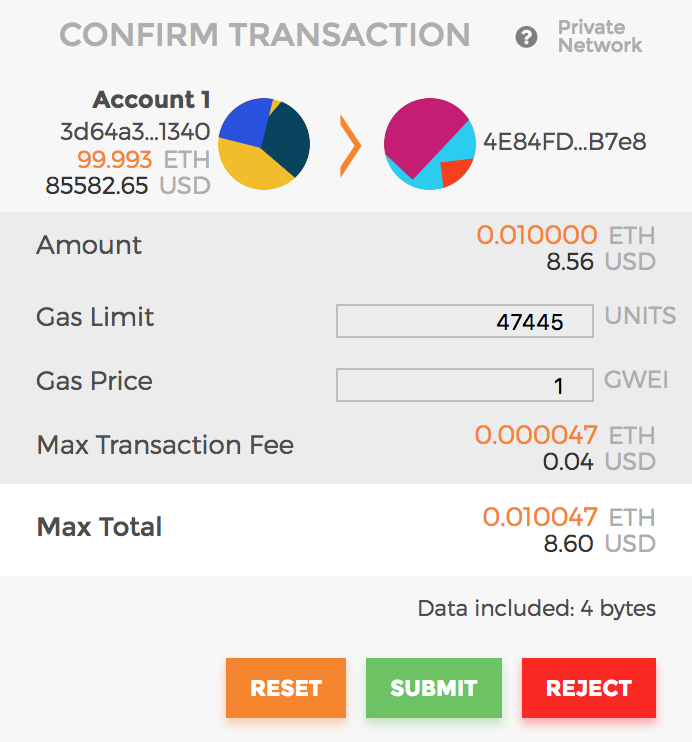
\includegraphics[width=\linewidth]{makebet}
  \caption{Making a bet using MetaMask}
\endminipage\hfill
\minipage{0.4\textwidth}
  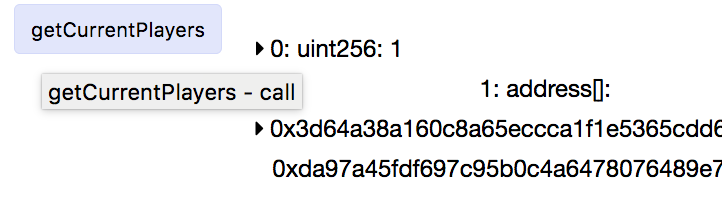
\includegraphics[width=\linewidth]{getplayers}
  \caption{Inspecting the current players in the game}
  \bigskip
  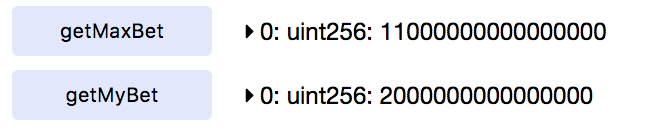
\includegraphics[width=\linewidth]{getbet}
  \caption{Inspecting the players current bet and the games max bet}
\endminipage\hfill
\end{figure}

\subsection{Failures}

Due to time limitations, a lack of Solidity programming experience, or other means, I experienced a number of failures while trying to implement this project.

\subsubsection{Randomness}

Randomness is a hot topic in the blockchain space. Obtaining unpredictable random numbers on the blockchain is difficult. A number of solutions exist or have been proposed \cite{random}, but I found it hard to successfully implement any one of them. I spent the most time attempting to implement a solution with Oraclize \cite{oraclize}, which was attractive for its ease of implementation. Developing with Oraclize became difficult, as it is a paid service and requires a connection to the main network (I was only working on my test network). Should this implementation had worked, the implementation would have relied on a third party service (and a centralised component).

Decentralised poker providers, Virtue \cite{virtue}, achieve randomness using generators on the players local system, through a desktop client. Since I was not building a front-end, I did not have the luxury of this.

The result of failure to provide randomness (and difficulties with looping over the deck to shuffle it, a failure in (understanding) Solidity \cite{shuffling}) resulted in the game being played with an unshuffled deck, leaving the game predictable and therefore not suitable for play with real stakes.

\subsubsection{Secrecy}

In the time frame, and given the complexity of the project, I failed to implement any form of secrecy. This would have been important for encrypting values such as the deck and the players hands (and could have been solved by encrypting each card individually). However, given the lack of randomness in shuffling the deck, I did not reach a point where implementing secrecy was important. Successfully implemented features, such as betting and round iterations, required no form of secrecy.

\subsubsection{Stack Limitations}

Due to stack limitations in Solidity \cite{stack}, implementing the algorithms to determine the winner required a number of refactors \cite{stackrefactor}. The refactors involved removing the number of local variables, to reduce the amount of information stored on the stack.

However I was unable, for unknown reasons, to implement the \texttt{hasTwoPair} function, which determines whether the player holds two distinct pairs between his hand and the table. I attempted to implement this function in a number of different ways, but at each attempt creating the contract would fail with an infinite gas cost warning.

%\subsubsection{Card Mappings}
%
%I attempted to map card numbers (0..51) to legible values, such as "2C" for the two of clubs. To implement this I chose to store and populate a mapping of \texttt{uint}, representing the card number, to \texttt{string}, containing the legible value. I ran into Solidity's inability to store dynamic arrays (the \texttt{mapping}) of dynamic arrays (the \texttt{string}). I could have solved this problem by reimplementing the mapping as a fixed length array of strings, \texttt{string[52]}, but did not due to time constraints.